\section{Community Earth System Model (CESM)}
\label{sec:cesm}

\subsection{Introduction}

Community Earth System Model (CESM) is a coupled global climate model simulating the earth system consisting ice, land, ocean, atmospheric and other components \cite{CESM:Hurrell}. In order to provide flexibility in developing, models in CESM do not communicate directly with each other but via a coupler. The Figure \ref{fig:mct} shows the communication between 4 models: Atmosphere (ATM), Ice (ICE), Land (LND) and Ocean (OCN) with the Coupler (CPL).

\begin{figure}[!htb]
\vspace{-0.15in}
\centering
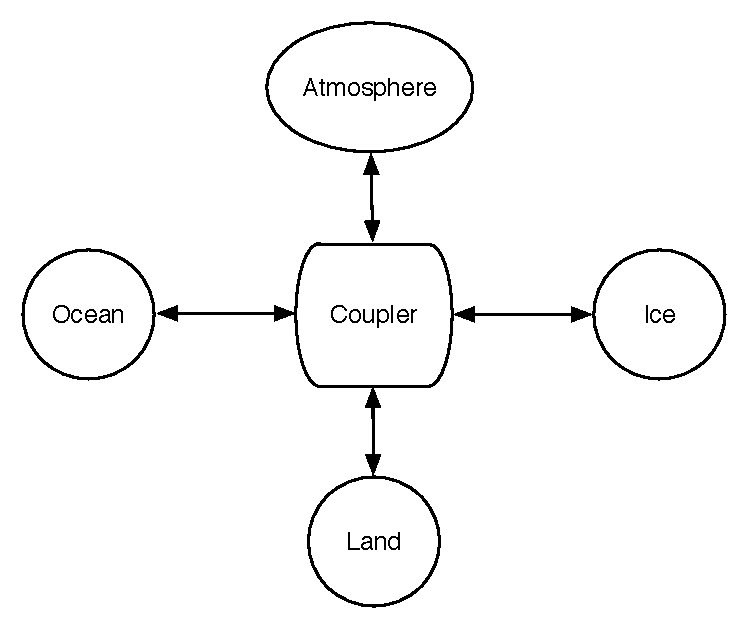
\includegraphics[scale=0.5]{figures/mct.pdf}
\vspace{-0.15in}
\caption{Model communicate with each other via a coupler}
\vspace{-0.15in}
\label{fig:mct}
\end{figure}

In this paper, we demonstrate the efficacy of our framework via communication between the models and the coupler extracted from a real run of CESM.

\subsection{Experiments and results}

Our experiment was carried on a partition of 512 nodes with 4 MPI/PAMI ranks per node. The positions of each component, and number of pairs of communication by rank and by node are shown in Table \ref{table:cesm_pair}

\begin{table}[!htbp]
   \centering
    \begin{tabular}{| l | c | r | r |}
    \hline
     \multirow{2}{*}{Model} & \multirow{2}{*} {Location} & \multicolumn{2}{ c| }{Num. of pairs of communication with Coupler} \\ \cline{3-4}
     & & Between Ranks & Between Nodes \\ \hline
     ATM & 0 - 1791 & 5227 & 2911 \\ \hline
     LND & 0 - 515 & 10390 & 2911\\ \hline
     ICE & 516 - 1791 & 3018 & 765 \\ \hline
     OCN & 1792 - 2047 & 2001 & 502 \\ \hline
     CPL & 0 - 1791 & & \\ \hline
    \end{tabular}
    \caption{Locations and number of pairs of communication between models in CESM}
    \label{table:cesm_pair}
\end{table}

The Table \ref{table:cesm_pair} shows the ranges of ranks (start-end) that host the models and the coupler. It also shows the number of pairs of communication between the models and the coupler.



We carried out the experiments communication between Coupler with Atmosphere, Land and Ocean.
The result of the expriment is shown in Table \ref{table:cesm_results} for 3 pairs of communication between CPL-ATM, CPL-LND and CPL-OCN. The throughputs are shown for different approaches Optmization (OPT), Heurisic (HEU) and MPI\_Alltoallv (MPI). We also show the total number of paths and the maximum, average number of paths per job for each approach.

\begin{table}[!htbp]
   \centering
    \begin{tabular}{| l | l | r | r | r | r |}
    \hline
    \multirow{3}{*}{Coupling} & \multirow{3}{*}{Type} & \multirow{3}{1cm}{BW (GB/s)} & \multicolumn{3}{ c| }{Num. of Paths} \\ \cline{4-6}
    & & & \multirow{2}{0.5cm}{Total Paths} & \multicolumn{2}{ c| }{Per Job} \\ \cline{5-6}
    & & & & {Max} & Avg \\ \hline
    \multirow{3}{*}{CPL-ATM} & OPT    & 352.24 & 3987 & 5 & 1.37 \\ \cline{2-6}
    & HEU & 327.66 & 15022 & 15 & 5.16 \\ \cline{2-6}
    & MPI    & 276.71 & 2911 & 1 & 1.00 \\ \hline
    \multirow{3}{*}{CPL-LND} & OPT    & 343.5 & 4004 & 7 & 1.38 \\ \cline{2-6}
    & HEU &  332.40 & 15107 & 14 & 5.19 \\ \cline{2-6}
    & MPI    & 278.90 & 2911 & 1 & 1.00 \\ \hline
    \multirow{3}{*}{CPL-OCN} & OPT    & 135.16 & 987 & 5 & 1.97 \\ \cline{2-6}
    & HEU &  136.06 & 5924 & 35 & 11.80 \\ \cline{2-6}
    & MPI    & 104.44 & 502 & 1 & 1.00 \\ \hline
    \end{tabular}
    \caption{Throughput, total number of paths, number of paths per job for 3 couplings in 512 nodes (4 ranks/node) experiments.}
    \label{table:cesm_results}
\end{table}

As shown in the Table \ref{table:cesm_results}, Optimization approach usually has the highest throughput, except for the CPL-OCN case, where Optimization approach and Heuristic approach have similar performance. The Heuristic approach usually has the second highest throughput. MPI has the lowest throughput. This is because MPI uses only one path to transfer data between 2 nodes. This leads to sharing links between pairs of communication comming from the same source node to the same destination nodes. Also the routing policy does not consider idle links and load on neighboring to balance the load. Both the factors lead to low performance in MPI. Heuritic approach employs the most number of paths, but due to the data assignment is not as optimal as Optimization approach, it still has lower performance. With the performance improvment of $~$30\% we can see that by using multipath we can rebalance network load and improve communication throughput.

\begin{comment}
\begin{table*}[!htbp]
   \centering
    \begin{tabular}{| l | l | r | r | p{0.5cm} | p{0.5cm} | p{0.5cm} | p{0.5cm} |p{0.5cm} | p{0.5cm} |p{0.5cm} | p{0.5cm} |p{0.5cm} | p{0.5cm} |}
    \hline
    \multirow{3}{*}{Coupling} & \multirow{3}{*}{Type} & \multirow{3}{1cm}{BW (GB/s)} & \multicolumn{3}{ c| }{Num. of Paths} & \multicolumn{2}{ c| }{Hopbytes} & \multicolumn{2}{ c| }{Num of copies}& \multicolumn{2}{ c| }{Num of paths} & \multicolumn{2}{ c| }{Total data} \\ \cline{4-6}
    & & & \multirow{2}{0.5cm}{Total Paths} & \multicolumn{2}{ c| }{Per Job} & \multicolumn{2}{ c| }{Per Path (MB)} & \multicolumn{2}{ c| }{Per Path}& \multicolumn{2}{ c| }{Per Link}& \multicolumn{2}{ c| }{Per Link (MB)} \\ \cline{5-14}
    & & & & {Max} & Avg & Max & Avg & Max & Avg & Max & Avg & Max & Avg\\ \hline
    \multirow{3}{*}{CPL-ATM} & OPT    & 352.24 & 3987 & 5 & 1.37 & 72 & 20.61 & 480 & 128.50 & 20 & 5.21 & 44.62 & 22.81 \\ \cline{2-14}
    & HEU & 327.66 & 15022 & 15 & 5.16 & 12.90 & 1.37 & 162 & 17.22 & 75 & 16.73 & 13.18 & 5.00 \\ \cline{2-14}
    & MPI    & 276.71 & 2911 & 1 & 1.00 & 0.14 & 0.07 &  &  & 18 & 3.71 &  & \\ \hline
    \multirow{3}{*}{CPL-LND} & OPT    & 343.5 & 4004 & 7 & 1.38 & 70 & 20.85 & 448 & 130.54 & 18 & 5.24 & 44.62 & 22.77 \\ \cline{2-14}
    & HEU &  332.40 & 15107 & 14 & 5.19 & 12.90 & 1.36 & 168 & 17.12 & 75 & 16.81 & 13.31 & 5.00 \\ \cline{2-14}
    & MPI    & 278.90 & 2911 & 1 & 1.00 & 0.14 & 0.07 & 0 & 0.00 & 18 & 3.71 & 0 & 0 \\ \hline
    \multirow{3}{*}{CPL-OCN} & OPT    & 135.16 & 987 & 5 & 1.97 & 864 & 252.51 & 6048 & 1626.19 & 11 & 2.47 & 253.62 & 120.46\\ \cline{2-14}
    & HEU &  136.06 & 5924 & 35 & 11.80 & 157.06 & 9.98 & 2148 & 126.98 & 78 & 9.47 & 64.75 & 19.1346 \\ \cline{2-14}
    & MPI    & 104.44 & 502 & 1 & 1.00 & 0.14 & 0.07 & 0 & 0.00 & 9 & 3.12 & 0 & 0 \\ \hline
    \end{tabular}
    \caption{Throughput, total num of paths, number of paths per job, maximum and average values of hopbytes, number of copies, number of paths per link and amount of data per link for 3 couplings in 512 nodes (4 ranks/node) experiments.}
    \label{table:cesm_results}
\end{table*}
\end{comment}

